\documentclass[a4paper]{report}
\usepackage[utf8]{inputenc}
\usepackage{amssymb}
\usepackage{amsmath}
\usepackage[margin=1in]{geometry}
\usepackage{graphicx}
\usepackage{verbatim}
\usepackage{bm}
\usepackage{listings}

\lstset{
  basicstyle=\ttfamily,
  mathescape
}

\title{Models + datasets - Notes}
\author{André Oskar Andersen}
\date{}

\begin{document}
    
\maketitle

\chapter*{Mask R-CNN}
\section*{Abstract}
Our approach efficiently detects objects in an image while simultaneously generating a high-quality segmentation mask for each instance. 

\section*{1. Introduction}
Instance segmentation is challenging because it requires the correct detection of all objects in an image while also precisely segmenting each instance. It therefore combines elements from the classical computer vision tasks of object detection, where the goal is to classify individual objects and localize each using a bounding box, and semantic segmentation, where the goal is to classify each pixel into a fixed set of categories without differentiating object instances (we use \textit{object detection} to denote detection via \textit{bounding boxes}, not masks, and \textit{semantic segmentation} to denote per-pixel classification without differentiating instances. Yet we note that \textit{instance segmentation} is both semantic and a form of detection).
\\
\\
We found it essential to decouple mask and class prediction: we predict a binary mask for each class independently, without competition among classes, and rely on the network's RoI classification branch to predict the category.
\\
\\
Finally, we showcase the generality of our framework via the task of human pose estimation on the COCO keypoint dataset. By viewing each keypoint as a one-hot binary mask, with minimal modification Mask R-CNN can be applied to detect instance--specific poses.

\section*{3. Mask R-CNN}
We behin by briefly reviewing the Faster R-CNN detector. Faster R-CNN consists of two stages. The first stage, called Region Proposal Network (RPN), proposes candidate object bounding boxes. The second stage, which is in essence Fast R-CNN, extracts features using RoIPool from each candidate box and performs classifcation and bounding-box regression. 
\\
\\
Mask R-CNN adopts the same two-stage procedure, with an identical first stage (which is RPN). In the second stage, in parallel to predicting the class and box offset, Mask R-CNN also outputs a binary mask for each RoI. This is in contrast to most recent systems, where classification depends on mask predictions. Our approach follows the spirit of Fast R-CNN that applies bounding-box classification and regression in parallel (which turned out to largely simplify the multi-stage pipeline or original R-CNN).
\\
Formally, during training, we define a multi-task loss on each sampled RoI as $L = L_{cls} + L_{box} + L_{mask}$. The classification loss $L_{cls}$ and bounding-box loss $L_{box}$ are identical as those defined in the Fast R-CNN paper. The mask branch has a $Km^2$-dimensional output for each RoI, which encodes $K$ binary masks of resolution $m \times m$, one for each of the $K$ classes. To this we apply a per-pixel sigmoid, and efine $L_{mask}$ as the average binary cross-entropy loss. For an RoI associated with ground-truth class $k$, $L_{mask}$ is only defined on the $k$-th mask (other mask outputs do not contribute to the loss).
\\
Our definition of $L_{mask}$ allows the network to generate masks for every class without competition among classes; we rely on the dedicated classifcation branch to predict the class label used to select the output mask. This decouples mask and class prediction.
\\
\\
\textbf{Mask Representation}: Specifically, we predict an $m \times m$ mask fro meach RoI using an FCN (fully convolutional network). This allows each layer in the mask branch to maintain the explicit $m \times m$ object spatial layout spatial dimensions. Unlike previous methods that resort to $fc$ layers for mask prediction, our fully convolutional representation requires fewer parameters, and is more accurate as demonstrated by experiments.
\\
\\
This pixel-to-pixel behavior requires our RoI features, which themselves are small feature maps, to be well aligned to faithfully preserve the explicit per-pixel spatial correspondence. This motvaited us to develop the following \textit{RoIAlign} layer that plays a key role in mask prediction.
\\
\\
\textbf{RoIAlign}: RoIPool is a standard operation for extracting a small feature map (e.g., $7 \times 7$) from each RoI. The quantization used by these operations introduce misalignments between the RoI and the extracted features. While this may not impact classification, it has a large negative effect on predicting pixel-accurate masks.
\\
To address this, we propose an RoIAlign layer that removes the harsh quantization of RoIPool, properly aligning the extracted fgeatures with the input. RoIAlign leads to large improvements.
\\
\\
\textbf{Network Architecture}: To demonstrate the generality of our approach, we instantiate Mask R-CNN with multiple architectures.

\section*{5. Mask R-CNN for Human Pose Estimation}
Our framework can easily be extended to human pose estimation. We model a keypoint's location as a one-hot mask and adopt mask R-CNN to predict $K$ masks, one for each of $K$ keypoint types.
\\
\\
\textbf{Implementation Details}: We make minor modifications to the se gmentation system when adapting it for keypoints. For each of the $K$ keypoints of an instance, the training target is a one-hot $m \times m$ binary mask where only a single pixel is labeled as foreground. During training, for each visible ground-truth keypoint, we minimize the cross-entropy loss over an $m^2$-way softmax output. We note that as in instance segmentation, the $K$ keypoints are still ttreated independently.

\chapter*{Understanding Mask R-CNN Basic Architecture}
\begin{figure}[h]
    \centering
    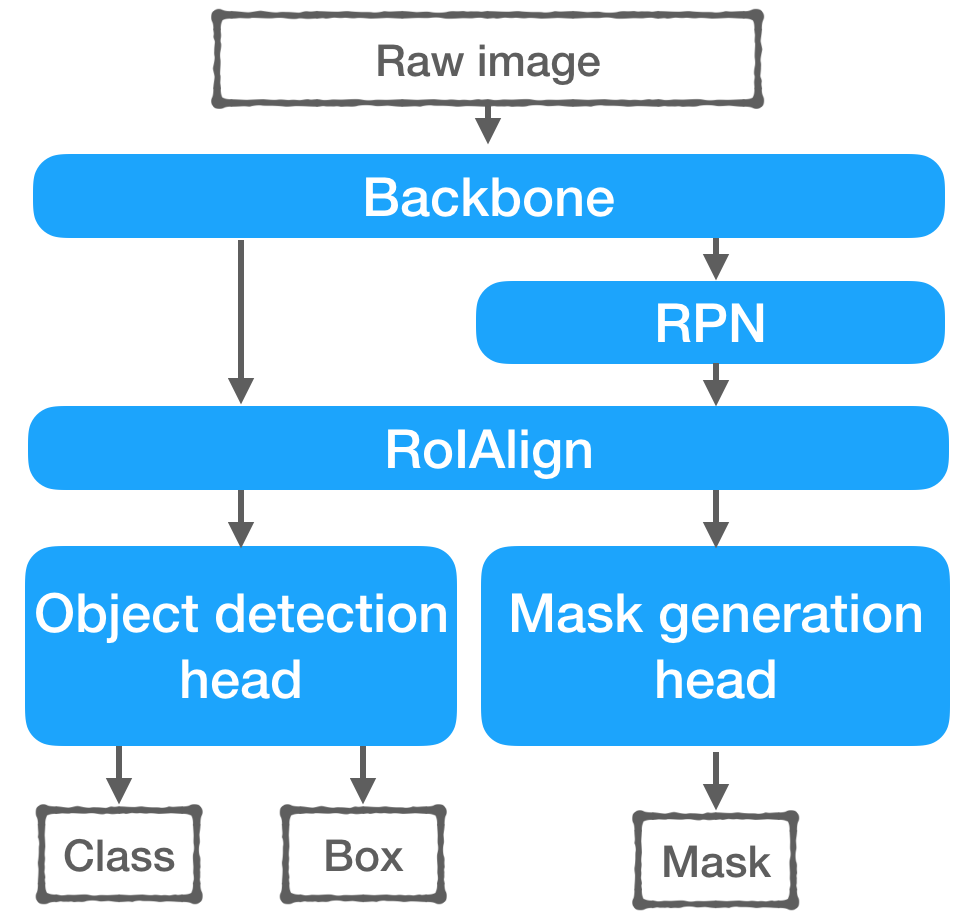
\includegraphics[width=0.4 \textwidth]{./entities/maskrcnn-big-picture.png}
    \caption{Overall Mask R-CNN architecture}
    \label{fig:RCNN_overall}
\end{figure}
Mask R-CNN is a popular deep learning framework for instance segmentation task in computer vision field. It adds fully convolutional networks (FCN) to Faster R-CNN to generate mask for each object.
\\
\\
Mask R-CNN can be composed by these parts: a backbone, a Region Proposal Network (RPN), a Region of Interest alignment layer (RoIAlign), a bounding-box object detection head and a mask generation head. The ove rall structure can be illustrated as in Figure \ref{fig:RCNN_overall}

\section*{1. Backbone}
\begin{figure}[h]
    \centering
    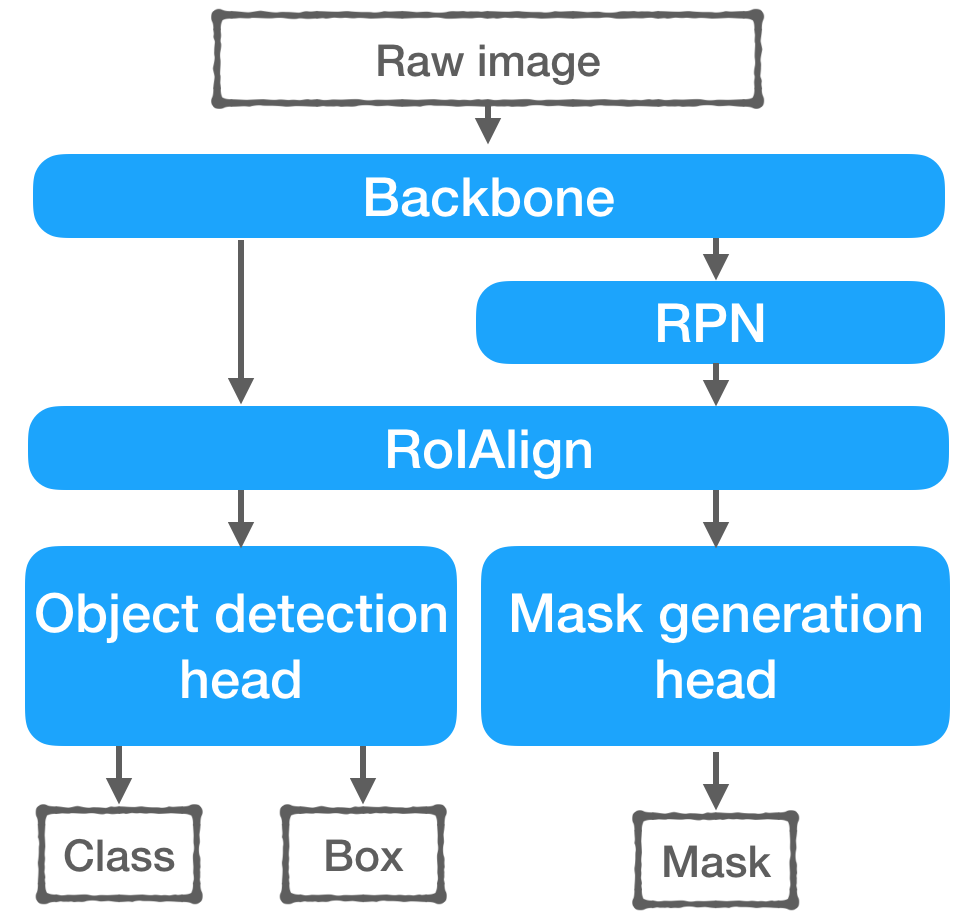
\includegraphics[width=0.4 \textwidth]{./entities/maskrcnn-big-picture.png}
    \caption{Mask R-CNN backbone}
    \label{fig:RCNN_backbone}
\end{figure}
A backbone is the main feature extractor of Mask R-CNN. When we feed a raw image into a backbone, data goes through blocks and turns into a feature map.
\\
\\
Feature map from the final convolutional layer of the backbone contains abstract informations of an image, e.g., different object instances, their classes and spatial properties. It is then fed to the RPN.

\section*{2. RPN}
\begin{figure}[h]
    \centering
    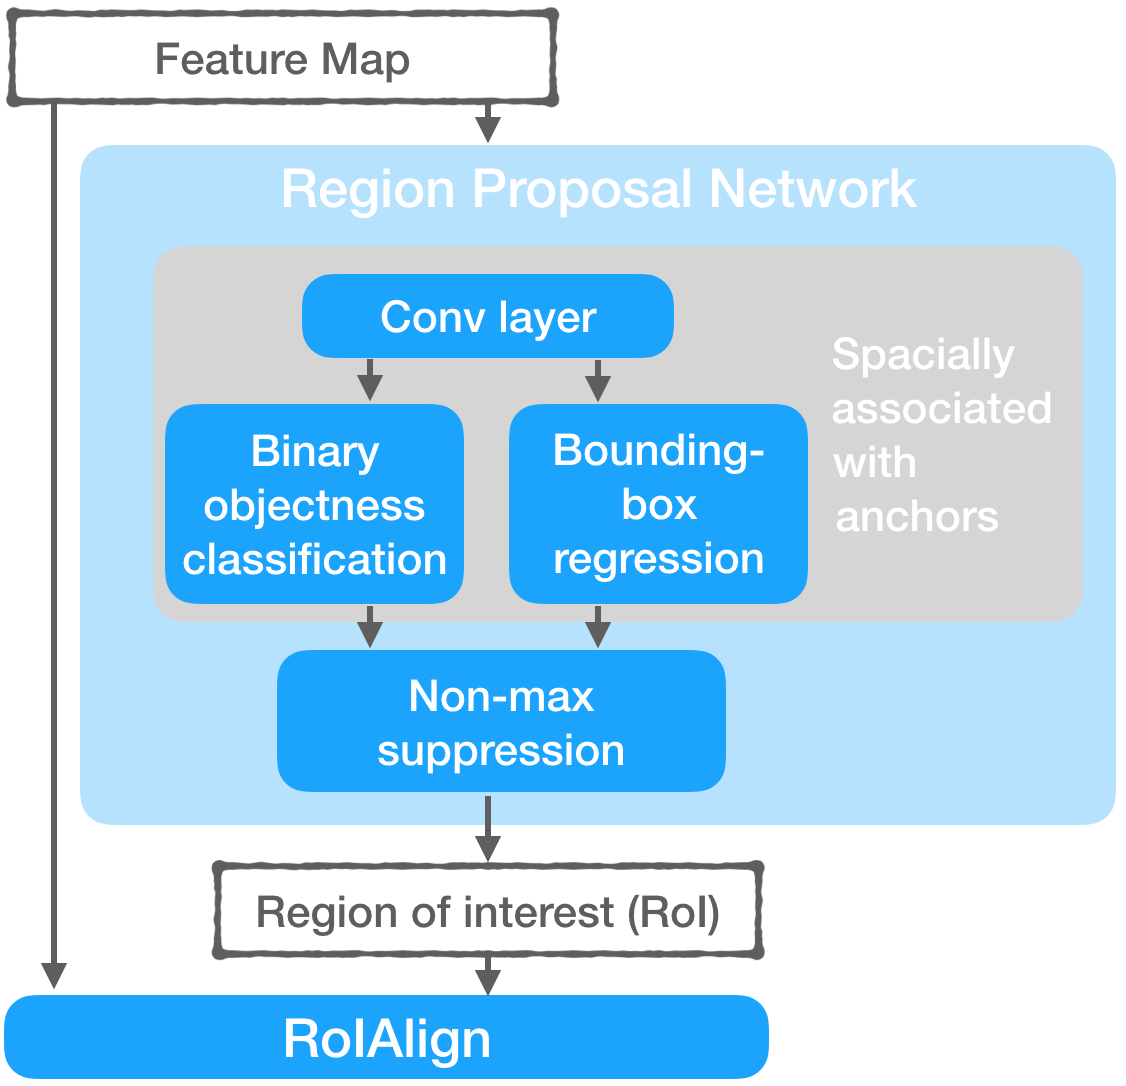
\includegraphics[width=0.4 \textwidth]{./entities/maskrcnn-rpn.png}
    \caption{Mask R-CNN RPN}
    \label{fig:RCNN_RPN}
\end{figure}
The function of RPN is to scan the feature map and propose regions that may have objects in them (Region of Interest or RoI). As so, we get a bunch of proposed RoIs. The next step is to find where exactly each RoI is in the feature map. It's called RoIAlign.

\section*{3. RoIAlign}
\begin{figure}[h]
    \centering
    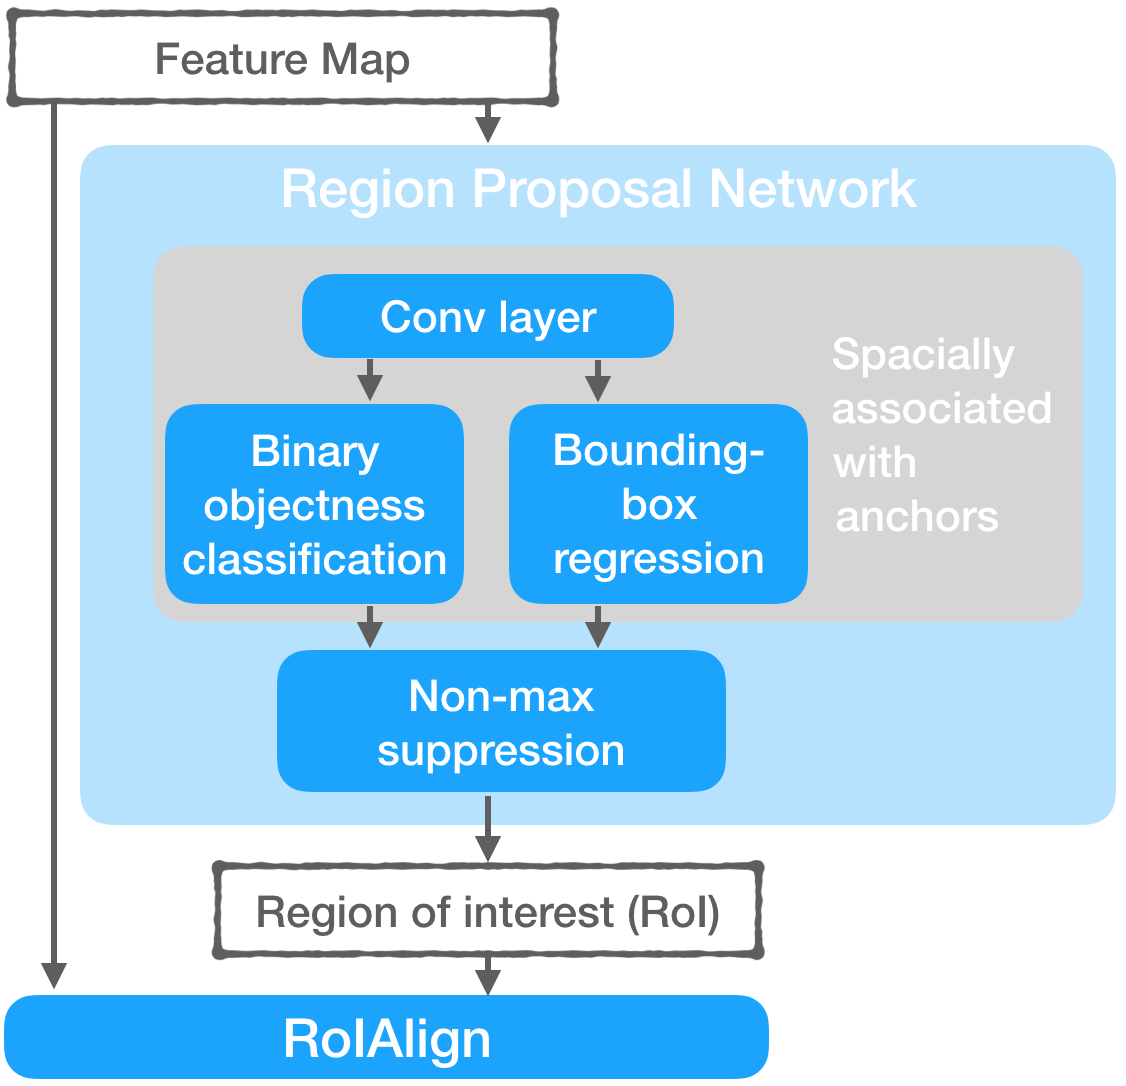
\includegraphics[width=0.4 \textwidth]{./entities/maskrcnn-rpn.png}
    \caption{Mask R-CNN RoIAlign}
    \label{fig:RCNN_RoIAlign}
\end{figure}
RoIAlign or Region of Interest alignment extracts feature vectors from a feature map based on RoI proposed by RPN, and turn them into a fix-sized tensor for further processes. The results represent every RoI's finer feature map and will be processed by two following parallel branches: object detection branch and mask generation branch.

\section*{4. Object detection branch}
\begin{figure}[h]
    \centering
    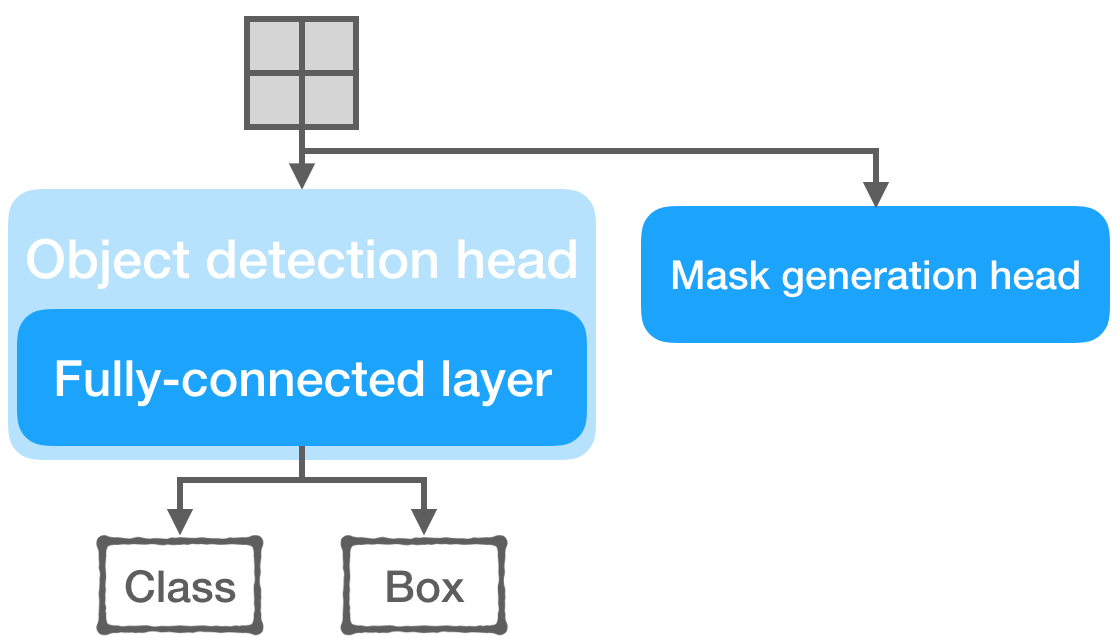
\includegraphics[width=0.4 \textwidth]{./entities/maskrcnn-object-detection-head.png}
    \caption{Mask R-CNN Object Detection Branch}
    \label{fig:RCNN_ODB}
\end{figure}
After we get individual RoI feature map, we can predict its object category and a finer instance bounding-box. This branch is a fully-connected layer that maps feature vectors to the final n classes and 4n instance bounding-box coordinates

\section*{5. Mask Generation Branch}
\begin{figure}[h]
    \centering
    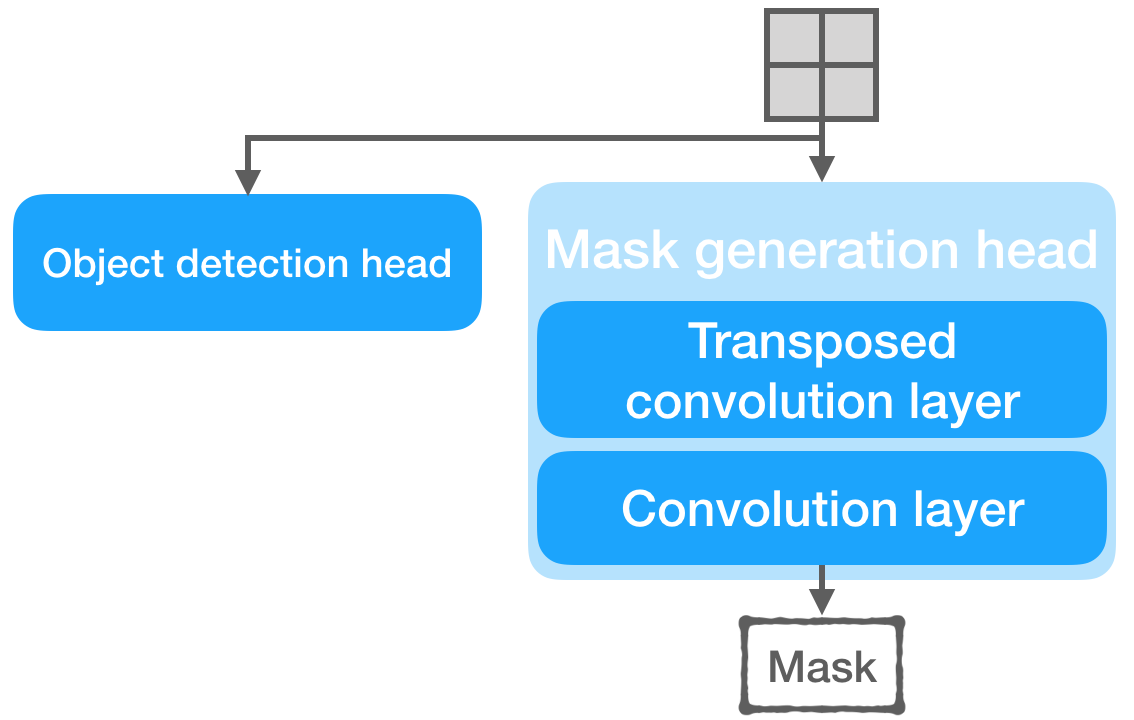
\includegraphics[width=0.4 \textwidth]{./entities/maskrcnn-mask-head.png}
    \caption{Mask R-CNN Mask Generation Branch}
    \label{fig:RCNN_MGB}
\end{figure}
On the mask generation branch, we feed RoI feature map to a transposed convolutional layer and a convolutional layer successively. This branch is a fully convolutional network. One binary segmentation mask is generated for one class. Then we pick the output mask according to the class prediction in object detection branch. In this way, per-pixel's mask prediction can avoid competition between different classes.

\chapter*{UniPose: Unified Human Pose Estimation in Single Images and Videos}
\section*{Abstract}
Our method is extended to UniPose-LSTM for multi-frame processing and achieves state-of-the-art results for temporal pose estimation in video. 

\begin{figure}[h]
    \centering
    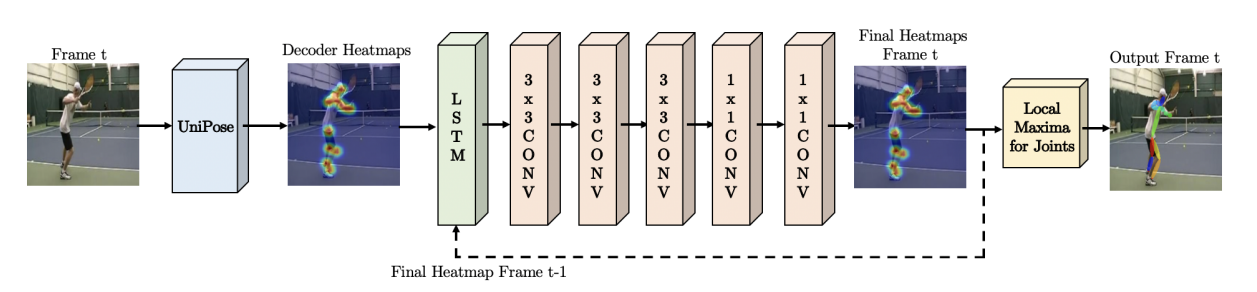
\includegraphics[width=0.8 \textwidth]{./entities/unipose.PNG}
    \caption{UniPose-LSTM architecture}
    \label{fig:Unipose}
\end{figure}
The UniPose architecture was modified to UniPose-LSTM for pose estimation in video. For video processing, it is useful to leverage the similarities and temporal correlation between consecutive frames.
\\
To operate in video processing mode, the UniPose architecture is augmented by an LSTM module that receives the final heatmaps from the previous frame along with the decoder heatmaps from the current frame. This network includes CNN layers following the LSTM to generate the final heatmaps used for joint detection.
\\
It was experimentally determined that accuracy impro ves when incorporating up to 5 frames in the LSTM, and a plateau in accuracy was observed for additional frames.

\section*{4. Datasets}
For video, two datasets are used: Penn Action and BBC Pose.
\\
Pen Action dataset contains 2,326 video sequences of 15 different activities including different sports, athletic acitivies, and playing instruments. The dataset was used to evaluate the performance of our architecture for temporal pose estimation and joint tracking.
\\
The BBC Pose dataset consists of 20 video from BBC. The BBC Pose dataset was utilized for the spcialized application of human pose for sign language.

\chapter*{LSTM Pose Machines}
\begin{figure}[h]
    \centering
    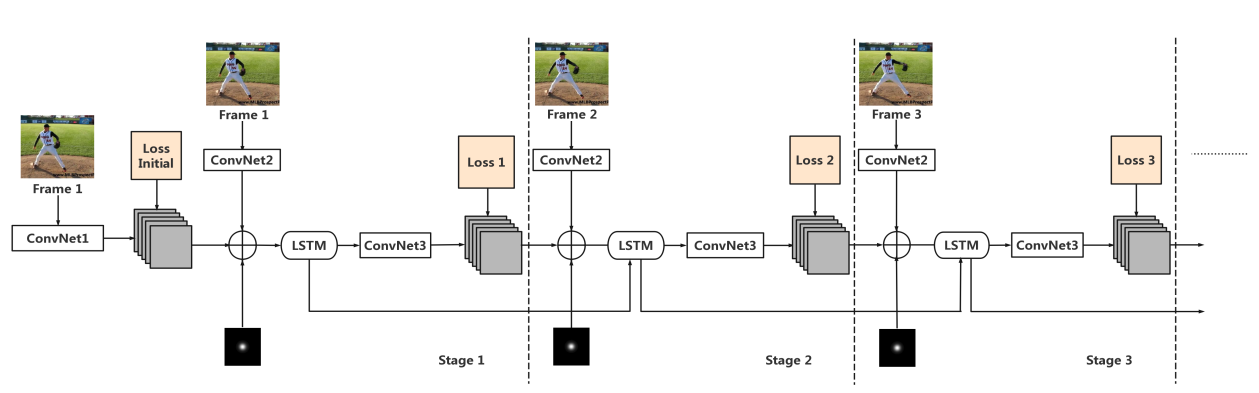
\includegraphics[width=0.8 \textwidth]{./entities/LSTM_pose_machine.PNG}
    \caption{Network architecture for LSTM Pose Machines}
    \label{fig:LSTM_pose_machine}
\end{figure}
\subsection*{3.2. LSTM Pose Machines}
\textbf{Details of the Model}.
Figure \ref{fig:LSTM_pose_machine} illustrates the structure for pose estimation on video.

\section*{3. Analysis and Our Approach}
\subsection*{3.1. Pose Machines: From Image to Video}
We add an extra slice containing a central gaussian peak during input concatenation for better performance.

\subsection*{4.1. Datasets}
JHMDB is a video-based dataset for pose estimation.

\chapter*{Detect-and-Track: Efficient Pose Estimation in Videos}

\section*{3. Technical Approach}
We propose a two-stage approach that efficiently and accurately tracks human instances and their poses across time. We build a 3D human pose predictor by extending Mask R-CNN with spatiotemporal operations by inflating the 2D convolutions into 3D. Our model takes as input short clips and predicts the poses of all people in the clips by integrating temporal information. We show that our 3D model outperforms its 2D frame-level baseline for the task of pose estimation. To track the instances in time, we perform a lightweight optimization that links the prediction. 

\subsection*{3.1 Two-Stage Approachy for Pose Tracking}
\begin{figure}[h]
    \centering
    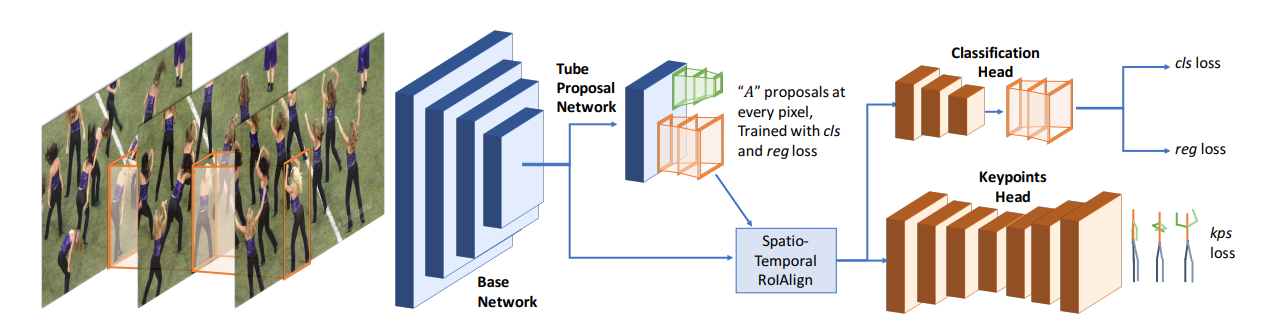
\includegraphics[width=0.8 \textwidth]{./entities/Detect_and_track.PNG}
    \caption{Network architecture for Detect and track}
    \label{fig:Detect_and_track}
\end{figure}
\subsection*{3.1. Two-Stage Approach for Pose Tracking}
\subsubsection*{Stage 1: Spatiotemporal pose estimation over clips.}
The first stage in our two-stage approach for human keypoint tracking is pose estimation using a CNN-based model. For this work we use Mask R-CNN due to its simple formulation and robust performance. 
\\
\\
Starting fro mthe vanilla Msk R-CNN model, we transform the 2D convolutions to 3D. Now, the input to our model is no longe a single frame, but a clip of length $T$ composed of adjacent frames sourced from a video. We extend the region proposal network (RPN), to predict object candidates which track each hypothesis across the frames of the input clip. The features are then fed into the 3D CNN head responsible for pose estimation. 
\\
\\
\textbf{Base network:} We extend a standard ResNet architecture to a 3D ResNet architecture by replacing all 2D convolutions with 3D convolutions. We initialize the 3D ResNet using a pretrained 2D ResNet.
\\
\\
\textbf{Tube proposal network}: We designa  tube proposal network inspired by the region propsal network (RPN) in Faster R-CNN. Given the featurem pa from the base network, we slide a small 3D-conv network connected to sibling fully connected layers.
\\
\\
\textbf{3D Mask R-CNN heads}: Given the tube candidates produced by the tube proposal network, the next step classifies and regresses them into a tight tube around a person track. We compute the region features for this tube by designing a 3D region transform operator.

\subsubsection*{Stage 2: Linking keypoint predictions into tracks}
Given the keypoint predictions grouped in space by person identity, we need to link them in time to obtain keypoint tracks. Tracking can be seen as a data association problem over these detections. We represent these detections in a graph, where each detection bounding box in a frame becomes a nod. We define edges to connect each box in a frame to every box in the next frame.

\subsubsection*{4.1. Dataset and Evaluation}
PoseTrack is a recently released large-scale challenge dataset for human body keypoint estimation and tracking in diverse, in-the-wild videos.

\chapter*{Flowing ConvNets}
\begin{figure}[h]
    \centering
    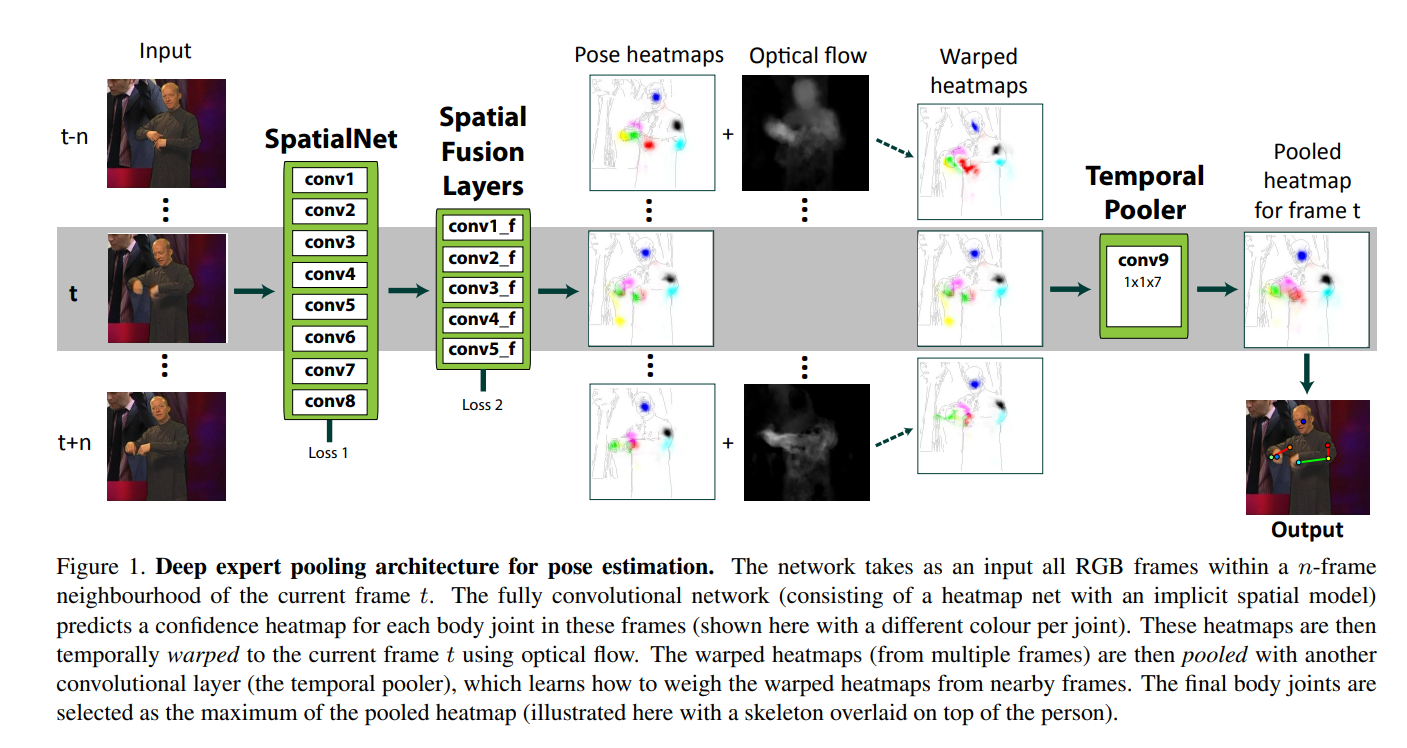
\includegraphics[width=0.8 \textwidth]{./entities/flowing_convnets.PNG}
    \caption{Network architecture for Flowing ConvNets}
    \label{fig:Flowing_ConvNets}
\end{figure}

\section*{4. Datasets}
\textbf{BBC Pose dataset}. This dataset consists of 20 videos (each 0.5h - 1.5h in length) recorded fro mthe BBC with an overlaid sign language interpreter. Each frame ehas been assigned pose estimates using the semi-automatic but reliable pose estimator of Buehler et al. 1,000 frames in the dataset have been manually annotated with upper-body pose.
\\
\\
\textbf{Extended BBC Pose dataset}. This dataset contains 72 additional training videos, which, combined with the original BBC TV dataset, yields in total 85 training videos. The frames of these new videos have been assigned poses using the automatic tracker of Charles et al. The output of this tracker is noisier than the semi-automatic tracker of Buehler et al., which results in partially noisy annotations.
\\
\\
\textbf{ChaLearn dataset}. The ChaLearn 2013 Multi-modal gesture dataset contains 23 hours of Kinect data of 27 people. The data includes RGB, depth, foreground segmentations and full body skeletons. In this dataset, both the training and testing labels are noisy (from Kinect). The large variation in clothing across videos poses a challenging task for pose estimation methods.
\\
\\
\textbf{Poses in the Wild and FLIC datasets}. The Poses in the Wild dataset contains 30 sequences (total 830 frames) extracted from Hollywood movies. The frames are annotated with upper-body poses. It contains realistic poses in indoor and outdoor scenes, with background clutter, severe camera motion and occlusions.

\chapter*{3D Human Pose Estimation using Spatio-Temporal Networks with Explicit Occlusion Training}

\section*{Abstract}
During training, we explicitly mask out some keypoints to simulate various occlusion cases, from minor to severe occlusion, so that our network can learn better and becomes robust to various degrees of occlusion.

\section*{Introduction}
In order to deal with occlusion, during the training, we mask out some keypoints or frames by setting the corresponding heat maps to zero.

\section*{Data Augmentation for Occlusions}
To make our approach capable of dealing with different occlusion cases, we perform data augmentation during the training.
\\
We use random masking of keypoints to simulate the occluded condition. Three types of occluision are applied in the training process. The first type is the frame-wise occlusion. Given a sequence of heatmaps produced by the 2D keypoint estimator, we randomly mask several frames by setting their heatmaps to zero, indicating that the whole frame is occluded or has low confidence. Second, the point-wise occlusion is applied by randomly setting certain keypoints' heatmaps to zero. This simulates the scenario that certain keypoints are occluded. Third, we apply area occlusion by setting a virtual occluder area. The heatmaps of keypoints located within this area are set to zero.

\chapter*{Combining detection and tracking for human pose estimation in videos}
\section*{Introduction}
We detect person bounding boxes on each frame and then propagate these to their neighbours. Our intuition is that if a person is present at a specific location in a frame, they should still be at approximately that location in the neighbouring frames, even when the detector fails to find them.
\\
In details, given a localized person bounding box, we crop a spatial-tempoeral tube from the video centered at that frame and location. Then, we feed this tube to anovel Clip Tracking Network that estimates the locations of all the body joints of that person in all the frames ofthe tube. To solve this task, our Clip Tacking Network performs body joint detection and tracking simultaneously. This has two benefits: (i) by solving these tasks jointly, our network can better deal with unique poses and occlusions, and (ii) it can compensate for missed detections by predicting joints in all frames of the spatial-tempoeral tube, even for frames where the person was not detected. To construct this Clip Tracking network ,we extend the state-of-the-art High-Resolution Network (HRNet) architecture to the task of tracking, using 3D convolutions that are carefuly designed to help learn the tempoeral correspondence between joints.
\\
The Clip Tracking Network operates on fixed length video clips.

\subsection*{3.1 Clip Tracking Network}
\textbf{HRNet for human pose estimation in images}. Given an image, this top-down approach runs a person detector on it, which outputs a list of axis-aligned bounding boxes, one for each localized person. Each of these boxes is independently cropped and fed into HRNet, which consists of four stages of four parallel subnetworks trained to localize all body joints of only the central person in the crop.
\\
The output of HRNet is a set of heatmaps, one for each body joint. 
\\
\textbf{3D HRNet for video pose estimation and tracking.} Our approach operates on short video clips. First, it runs a person detector on the center frame and obtains a list of person bounding boxes. Then, for each bounding box, it creates a tube by cropping the box region from all frames in the clip. Next, it feeds this tube to our video HRNet, which outputs a tracklet containing all the poses of person $p$ in all the frames of the thube.
\\
In order to help the network tackle this challenge, we do two things: (i) to account for fast moving people, we enlarge each bounding box by $25\%$ along both dimensions prior to creating a tube; and(ii) to allow the network to associate people between frames, we inflate the 2D convolutions in the first two stages of HRNet to 3D to help the network learn to track. 

\chapter*{Temporal Feature Alignment and Mutual Information Maximization for Video-Based Human Pose Estimation}
\section*{3. Our Approach}
\textbf{Preliminaries} To detect human poses from video frames, we first extract the bounding box of each individual person. This bounding box is then enlarged by $25\%$ to crop the same individual on a predefined window of neighboring frames. 
\\
\textbf{Method Overview} FAMI-Pose consists of two main modules, a global transformation module and a local calibration module. We first perform feature extraction the each frame. These features are then fed into our global transformation module, which learns the parameters of an affine transformation to obtain a coarsely aligned supporting frame feature. The frame features are then handed to the local calibration module, which performs pixel-wise deformation to produce finely aligned features. Fiannly, we aggregate all aligned supporting frame features and the key frame feature to obtain our enhanced feature. This is then apssed to a detection head that outputs pose estimations.

\subsection*{3.1 Feature Alignment}
Feature alignment starts wtih feature extraction, which is done with the HRNet-W48 network (SOTA method for image-based human pose estimation) as the backbone. The extracted features are then passed through a global transformation module and a local calibration module, to progressively align the extracted features.
\\
\textbf{Global Transformation} We observe that most failure cases for pose estimation in videos occur due to rapid movements of persons or cameras, which inevitably lead to large spatial shifts or jitters between neighboring frames. In order to align a supporting frame to the key frame, we design a glboal transformation module (GTM). The GTM computes spatial rearrangement parameters of glibal affine transformation to obtain a coarse preliminary alignment of supporting frame feeature with the key frame feature.
\\
\textbf{Lobal Calibration} The global transformation module produces a coarse alignment. We then design our local clibration module (LCM) to perform meticulous fine-tuning at a pixel-level, yielding finely aligned features.
\\
\textbf{Heatmap Generation} Ultimately, we aggregate over all final aligned supporting frame features and the key frame feature via element-wise addition to obtain the enhanced feature. This is then fed to a detection head to produce pose heatmap esitmations. By effectively leveraging tempoeral information from supporting frames through our coarse-to-fine alignment modules, our FAMI-Pose is more adept at tackling visual degeneration issues and therefore gives more accurate pose heatmaps.

\chapter*{Deep High-Resolution Representation Learning for Human Pose Estimation}
\section*{Abstract}
In this paper, we are interested in the human pose estimation problem with a focus onn learning reliable high-resolution representations.

\chapter*{High-Resolution Network: A universal neural architecture for visual recognition}
\section*{Application}
The HRNet is a universal architecture vor visual recognition. The HRNet has become a standard for human pose estimation.

\section*{Human Pose Estimation}
The comparison with ResNet-based methods, we can see, that HRNet outperforms ResNet in terms of estimation performance, parameter complexity, and computation complexity.

\chapter*{DeciWatch: A Simple Baseline for 10x Efficient 2D and 3D Pose Estimation}
\section*{Abstract}
DeciWatch uniformly samples less than 10\% video frames for detailed estimation, denoises the estiamted 2D/3D poses with an efficient Transformer architecture, and then accurately recovers the rest of the frames using another Transformer-based network.

\section*{Introduction}
To achieve highly efficient 2D pose estimation without the need of watching every frame in a video, we propose a novel framework based on the continuity of human motions, which conducts pose estimation only on sparsely sampled video frames. Poses of those sampled frames should be denoised before recovered, where we formulate the thre-step sample-denoise-recover framework.

\section*{Method}
\subsection*{Problem Definition and Overview}
The main target of this work is to set a baseline for efficient video-based pose estimation without compromising accuracy. We devise a three-step sample-denoise-recover flow to process video-based pose estimation efficiently and effectively. As adjacent frames usually contain redundant information and human motion is continuous, DeciWatch first samples a small percentage of frame and applies existing pose estimators theoreon to obtain the corresponding poses. However, recovering the full pose sequence from sparsely observed poses is challenging, especially when the poses are estimated by networks and often contain noise. Relying on a few poses to recover the entire sequence, the quality of sampled poses is the key. To tackle the challenge, we introduce two subnets, DenoiseNet and RecoverNet. Specifically, DenoiseNet refines sparse poses from pose estimator. Then RecoverNet performs motion recovery based on the refined sparse poses to recover the whole pose sequence, with the inuition that humans can perceive complete motion information through a small number of keyframes.

\subsection*{Getting Sampled Poses}
We use a uniform sampling that watches one frame in every $N$frame to select sparse frames $I^\text{sampled}$ as a baseline strategy. Due to the redundancy in consecutive frames and continuity of human psoes, a uniform sampling strategy under a certain ratio is capable of keeping enough information for recovery. Then we can estimation $I^\text{sampled}$ by any existing pose estimators to get sparse poses.

\subsection*{Denoising the Sampled Poses}
In our scenario, the sampled poses are obtained by single-frame pose estimators, inevitably leading to noisy, sparse poses. Consequently, the quality of sparse poses is crucial for motion recovery. Before recovering the full motion, we develop a denoising network to refine the sampled poses to clean poses. Due to the tempoeral sparseness and noisy jutters, the key designs of Denoise Net lie in two aspects: (i) A dynamic model for handling diverse possible pose noises; (ii) Global tempoeral receptive field to capture useful Spatio-tempoeral information while suppressing distracting noises. Based on these two considerations, local operations, like convolutional or recurrent networks, are not well suited. Intuitively, Transformer-based models are capable of capturing the global correlations among discrete tokens, so we use Transformer-based encoder modules to relieve noises from the sparse poses.

\subsection*{Recovering the Sampled Poses}
After getting the sparse clean poses, we use another Spatio-tempoeral subet, RecoverNet, to recover the absent poses. In order to learn the consistent tempoeral correlations, a simple tempoeral upsampling is applied to perform preliminary sequence recovery. To make the recovery more realistic and accurate, we adopt another transformer-based network for detailed poses recovery. We bring tempoeral semantics into pose encoding to encode the neighboring $D$ frames' poses into pose tokens via a tmepoeral 1D convolutional layer. The main architecture of RecoverNet is also the same as Transformer, which employs $M$ multi-head self-attention blocks

\chapter*{SportsCap: Monocular 3D Human Motion Capture and Fine-grained Understanding in Challenging Sports Videos}


\chapter*{Datsets}
\section*{PoseTrack2017/PoseTrack2018}
\begin{itemize}
    \item Multi-person pose estimation and tracking in videos.
    \item 512 videos including 6,374 frames in total.
    \item 30 frames from the center are annotated.
    \item 15 keypoint location
\end{itemize}

\section*{BBC Pose dataset}
\begin{itemize}
    \item 20 videos, each 0.5h - 1.5h
    \item Only upper body
\end{itemize}

\section*{Extended BBC Pose dataset}
\begin{itemize}
    \item 72 videos. 
    \item Only upper body
    \item Partially nopisy annotations
\end{itemize}

\section*{Poses in the Wild}
\begin{itemize}
    \item Multi-person pose estimation and tracking in videos.
    \item 51.000 frames
    \item Changing and cluttered backgrounds, as well as frequent occlusions.
    \item 18 keypoint locations
\end{itemize}

\section*{Human3.6M Dataset}
\begin{itemize}
    \item 3.6 million human poses in 3D
    \item 32 joints
\end{itemize}

\section*{Penn Action}
\begin{itemize}
    \item 2.326 video sequence.
    \item Single person
    \item 13 Keypoints
\end{itemize}

\section*{BRACE}
\begin{itemize}
    \item 334,538 Frames - 26,676 manually annotated frames
    \item 465 Video sequences
    \item 17 keypoints
\end{itemize}

\section*{SMART}
\begin{itemize}
    \item 5,000 video sequnces
    \item 2.1M frames
\end{itemize}

\end{document}